\documentclass[12pt]{article}
\usepackage[utf8]{inputenc}
\usepackage[russian]{babel}
\usepackage{multicol}
\usepackage[papersize={19cm, 33cm}, left=5mm, top=5mm, right=5mm, bottom=15mm]{geometry}
\usepackage{mathtools}
\documentclass[captions=tableheading]{scrbook}
\usepackage{caption}
\usepackage{tikz} 
\usepackage{amsmath}
\usepackage{graphicx}
\usepackage{wrapfig}
\graphicspath{{pictures/}}
\usepackage[usenames]{color}
\usepackage[most]{tcolorbox}
\usepackage{colortbl}
\usepackage{fancyhdr}
\usepackage{float}
\usepackage[leftcaption]{sidecap}
\setlength{\columnsep}{1cm}
\DeclareGraphicsExtensions{.png}
\usepackage{afterpage}
\fancypagestyle{mystile}{
\fancyhf{}
\fancyfoot[l]{\textbf{20}}
\renewcommand{\headrulewidth}{0pt}
\fancyhead{}
}
\pagestyle{mystile}

\begin{document}
\begin{multicols}{2}
\begin{flushleft}
\section*{§ 1. Что такое\\ многоугольник Ньютона}
\textbf{Диаграмма Ньютона\\многочлена от двух переменных}

Напомним, что \textit{одночленом} от неза-\\ 
висимых переменных х и у называ-\\
ется функция вида $x^{m} y^{n}$, где m и n -\\
неотрицательные целые числа, а мно-\\
гочленом от х и у с действительными\\
коэффициентами называется функция\\
Р (х, у), заданная формулой
\begin{equation}
P (x, y) = a_{1}O_{1} + a_{2}O_{2} + ... + a_{k}O_{k},
\end{equation}
где $a_{1}, a_{2}, ..., a_{k}$ - действительные\\
числа, а $O_{1}, O_{2}, ..., O_{k}$ - попарно\\
различные одночлены\footnote{)Независимые переменные х и у при-\\
нимают значения в множестве действитель-\\
ных чисел; таким образом, функция Р (х, у)\\
имеет в качестве области определения чис-\\
ловую плоскость, а в качестве множества\\
значений - числовую прямую.}). Если в фор-\\
муле (1) коэффициент $а_{i}$ отличен от\\
нуля, то говорят, что одночлен О_{i}\\
\textit{входит} в многочлен Р (х, у). Напри-\\ 
мер в многочлен $2+3y-\sqrt{2x^{3}y^{2}}$\\
входят одночлены 1, у и $x^{3}y^{2}$, a в\\
многочлен Р (х, у)$\equiv0$ не входит ни\\
один одночлен. Удобно изображать\\
одночлены, входящие в многочлен\\
Р (х, у), точками на координатной\\
плоскости: мы отмечаем на этой пло-\\
скости точку М $(m_{0};n_{0})$, если одно-\\
член $х^{m_{0}}у^{n_{0}}$ входит B многочлен\\
Р (х, у). Тогда каждому ненуле-\\
вому многочлену Р (х, у) мы сопостав-\\
ляем конечное множество на пло-\\
cкости Оmn - будем обозначать его\\
Д(Р), - изображающее наглядно од-\\
ночлены, входящие в Р (х, у). Точку\\
плоскости, у которой обе координа-\\
ты - целые числа, мы будем называть\\
\textit{целой} точкой. Для любого многочлена\\
Р множество Д (Р) состоит только\\
из целых точек, поэтому его удобно\\
рисовать на клетчатой бумаге. На-\\
пример, множество Д (Р) для много-\\
члена
\begin{equation}
P (x, y) = xy-y^{3}+ 3 x^{3}y^{2} +0,5х^{4} - 2x^{3}y^{4}
\end{equation}
изображено на рисунке 1. Подчерк-\\
нем, что значения ненулевых коэф-\\
фициентов многочлена Р никак не\\
учитываются при построении мно-\\
жества Д (Р). Это множество обычно\\
называют \textit{диаграммой Ньютона} мно-\\
гочлена Р.
\end{flushleft}

Предостережение. Не следует\\
смешивать числовую плоскость \textbf{R} - об-\\
ласть определения многочлена Р, с коорди-\\
натной плоскостью Omn, на которой мы ри-\\
суем диаграмму Ньютона многочлена Р.\\
Точки этих плоскостей имеют разную при-\\
роду.

\begin{flushleft}
\textbf{\footnotesizeКак Ньютон определял\\«диаграмму Ньютона»}
\end{flushleft}

Ньютон тоже отмечал одночлены,\\
входящие в многочлен от переменных\\
х, у, на клетчатой бумаге. Ньютон\\
расчерчивал такую бумагу сам и от-\\
мечал не углы клеток, а целые клетки.\\
Вот как он описывает эти построения\\
в письме одному из своих коллег.


«...Для лучшего уразумения это-\\
го правила поясню его на следующей\\
диаграмме. Построй прямой угол\\
ВАС; стороны его ВА и АС раздели\\
на равные части и, восставив перпен-\\
дикуляры, раздели угловую площадь\\
на равные квадраты или параллело-\\
граммы, которые отметь вписанными в\\
них измерениями букв х и у (см. ри-\\
сунок 2). Затем, когда дано уравне-\\
ние, отметь каким-нибудь знаком па-\\
раллелограммы, соответствующие\\
всем его членам...»

\begin{figure}[H]
    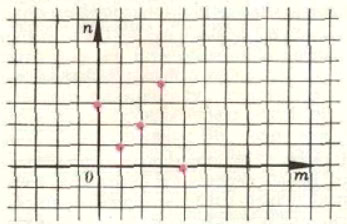
\includegraphics[scale=0.65]{рис1.png}
    \captionsetup{singlelinecheck=off}
    \caption{}
    \label{fig:ris6}
\end{figure}
\begin{figure}[H]
    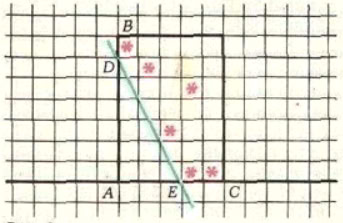
\includegraphics[scale=0.65]{рис2.png}
    \captionsetup{singlelinecheck=off}
    \caption{}
    \label{fig:ris6}
\end{figure}

\end{multicols}
\end{document}
